\documentclass[12pt,a4paper]{report}

\usepackage[utf8]{inputenc}
\usepackage[english]{babel}
\usepackage{amsmath}
\usepackage{amsfonts}
\usepackage{amssymb}
\usepackage{graphicx}
\usepackage{eurosym}
\usepackage[left=2cm,right=2cm,top=2cm,bottom=2cm]{geometry}
\usepackage{wrapfig}
\usepackage{mathdots}
\usepackage{caption}
\usepackage{cite}
\usepackage{mathrsfs}
\usepackage{float}
\usepackage{hyperref}

\author{Josep Maria Serra Moncunill}
\title{Critical failure}
\date{\today}


\begin{document}

\maketitle
\tableofcontents
\listoffigures
\listoftables

\section{Major failure deffinition}

\paragraph{}In Project Charter, it has been stated that a major failure can be defined as the loss of a client’s satellite coverage because of a failure in the network. However, this deffinition is not enough precise. For example, during a communication, it can happen that a data packet is lost, or has an error and it is discarded. This means that, for that packet, the communication was lost, but it dones not mean that the communication with the client was lost. Another aspect to take into account is that a satellite may fail, but an alternative path can still exist and, therefore, the communication can continue. Morover, if the client satellite loses all communication with all satellites in range, due to the different orbital velocities of the client satellite and the network satellites, the client satellite will eventually be in range of a functional network satellite.

\paragraph{}For all this reasons, a more specific criteria is needed. In Project Charter it has also been stated that the network will provide communication between a client satellite and a ground station with a latency lower than 5 minutes (300 seconds, or 300,0000 miliseconds). A major failure will consiste in a failure in the network that causes a message to arrive from a client satellite to a client ground station with more that 5 minutes of delay, or not arrive at all. Derived from this deffinition, a minor failure can also be deffined. It can be defined as a delay of more that 5 minutes in a communication between a client satellite and a ground station without any failure in the network.

\subsection{Major failure}

\paragraph{}Because of the different height of the client satellite and the network satellites, if all the network satellites is range of the client satellite fail, the client satellite may come in range of a working network satellite if enough time passes. In some cases, this can happen in less than 5 minutes and, therefore, it will not be considered a major failure. For this reason, a more critical situation will be considered. It will be considered that the client satellite moves at the same speed as the network satellites, in the same orbital plane. In this situation, a major failure can happen because for three reasons: all network satellites in range of the client satellite fail, all ground stations fail, or some satellites fail but the alternative path takes more that 5 minutes to transmit the information.

\subsubsection{Satellite in range failure}

\paragraph{}The first reason will be evaluation in the following lines. Depending on the location of the satellite and the distribution of the satellites in the constellation, the number of adjacent satellites may vary. A satellite over the ecuator can have up to six adjacent satellites. If a client satellite only communicates with this network satellite, a major failure will be the failure of this satellite, as it can be seen in Figure \ref{fig:critical1}. It can also be tha failure of a group of satellites surrounding the transmitting satellite, but this number is larger and, therefore, it would not be considered since the failure of the transmitting satellite is more restrictive.
\begin{figure}[H]
\begin{center}
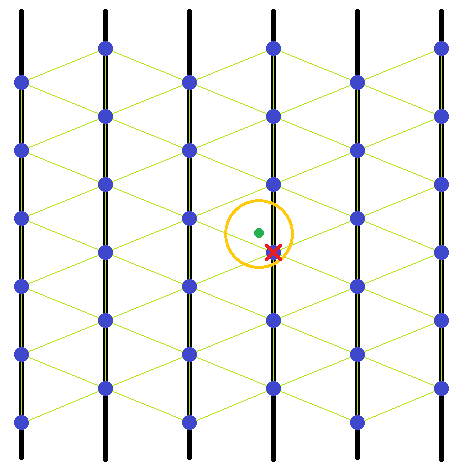
\includegraphics[scale=0.5]{critical1.PNG}
\caption[1 communication range failure]{Failure due to the loss of the only satellite in range of the client satellite.}
\label{fig:critical1}
\end{center}
\end{figure}
\paragraph{}For antennas with almost half-spherical patterns (an angle of 10º over their horizontal plane has been considered as the minimum angle capable of recieving and transmitting), the minimum height over the satellite network orbit in order to always see more than one satellite is, aproximately, 400 km, considering that our constellation is at 550 km height over the Earth's surface. This means that a significant portion of clients would be in that zone.

\paragraph{}For clients that have more than one network satellite in range, the critical failure would be similar as the ones in Figure \ref{fig:critical2} and Figure \ref{fig:critical3}. 
\begin{figure}[H]
\begin{center}
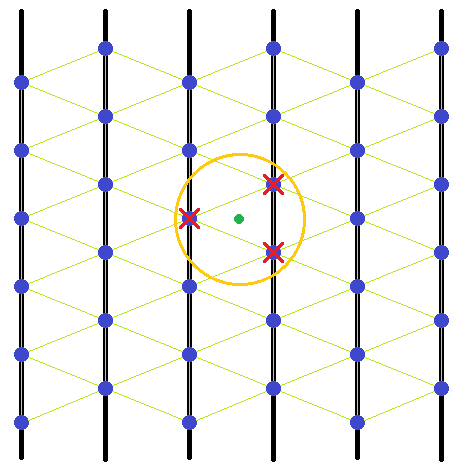
\includegraphics[scale=0.5]{critical2.PNG}
\caption[3 communication range failure]{Failure due to the loss of all possible communication satellites if the client can communicate to three network satellites.}
\label{fig:critical2}
\end{center}
\end{figure}
\begin{figure}[H]
\begin{center}
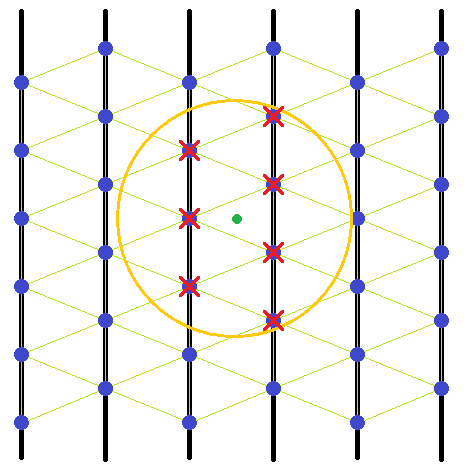
\includegraphics[scale=0.5]{critical3.PNG}
\caption[7 communication range failure]{Failure due to the loss of all possible communication satellites if the client can communicate to seven network satellites.}
\label{fig:critical3}
\end{center}
\end{figure}

\paragraph{}As it can be seen, the critical failure depends on the communication range of the client satellite. Taking the more restrictive one would mean considering the failure of only one satellite. As this affect a significant amount of potential clients, it can not be neglected.

\subsubsection{Ground station failure}

\paragraph{}Since any satellite in the network is able to communicate with any ground station, in order to have a critical failure due to a ground station failure, all ground stations must fail. It will not be considered a failure the loss of connection to a ground station caused by bad weather conditions or radio-fequency interference, since it is not a failure in the network but an anomaly in the medium.

\paragraph{}Therefore, for a critical failure caused by ground station failures to happen, all ground stations must fail. Since at least three ground stations will be used, the three of them must fail. As the previous case, the time of failure dones not matter, but the fact that they remain unoperative at a given time.

\subsubsection{Transmitting time failure}

\paragraph{}In the following lines, a major failure due to a delay supperior to 5 minutes originated by a failure will be evaluated. First of all, it is needed to evaluate the transmission time. The minimmum data rate that will handle the satellites is 25 Mbit/s. Therefore, it will be considered 25 Mbit/s as the data rate of the satellites, since it is the most restrictive. The protocols chosen, by deffault, cannot handle data units of more than 62,500 bytes, aproximately. This is 500.000 bits. With the data rate chosen, the time to transmit this information is 0.02 seconds. For a path of 20 nodes, and considering that a satellites recives the entire packet before sending it again, the transmission time will be 0.4 seconds. The transmission is done using electromagnetic waves, which move at the speed of light. For this short distances, it can be considered to be instantaneously. The time used to process each data packet has to be taken into account. If each node needs 1 second to process the packet, the total processing time will be 20 seconds. 

\paragraph{}Finally, the time to recognize a fallen satellite and the time to compute an alternative route is required. By deffault, OSPF protocol requires 40 seconds of no response to label an adjacent node as dead. When this time expires, the fallen link state will be transmitted. When a node recieves this update, it will wait 5 seconds and then it will calculate new routes. If the process requires 100 seconds, the total time until a failure happens and a new route is calculated is 145 seconds. With the processing time of 20.4 seconds, if one node fails, the time to deliver the message is 165.4 seconds. But if another node fails while the message is still being delivered, the total time to deliver the message would be 310.4 seconds, which is superior to 5 minutes.

\paragraph{}Therefore, for a critical failure to happen because of a delay of more than 5 minutes in the communication due to a failure in the network, two satellites must fail in less than 160 seconds, and both of them must be in a communication path between a client and a ground station.

\subsubsection{Conclusion}

\paragraph{}It can be concluded that a major failure can happen due to various factors:
\begin{itemize}
\item The failure of at one satellites.
\item The failure of all ground stations. It would be at least 3 ground stations.
\item The failure of at least two satellites in a communication route in less than 3 minutes.
\end{itemize}

\end{document}